\section{Environments}

% Section about environments and their performance
Environments - describe why simulated environments are used, what kind of
tasks they simulate, how they range in Accuracy, Performance, Complexity,
Usability.

In this section we will describe:
- What is the environment from RL perspective (state transition function, rewards).
- What are the examples of simulated environments (ALE, Mujoco, StarCraft).
- Why simulated environments are important for RL research? (Safe exploration, a lot of data,
adjustable complexity, well scoped skills testing, access to privilliged information).
- How simulated environments are commonly implemented, and what implication this brings?
(limited accuracy, limited speed, limited diversity (in case of opponents in board games))
- Which environments are used for benchmarking algorithms? (Atari, Mujoco).
- Other notable progress in environments development: DeepMind Lab, VizDoom, StarCraft 2.
- How this work addresses is connected to different environments: we build an adaptive algorithm,
that can take into account the speed of the environment.
- Tell more about environments used in this work: VizDoom.

%\section{FPS environment}
In this section we describe the FPS setup that we study in this work.
The player has control over the agent that lives in 3-dimensional environment, can perform several types of actions that influence this environment and has a goal that is dictated by the rules of the game.
As an input, agent receives 2-dimensional views of the environment from the first-person camera.

In our particular case there are 3 types of actions that agent can perform:
\begin{itemize}
    \item Movement --- moves the agent in the direction of specified 3-d vector. This command will be processed by the environment to account for possible obstacles and physical laws that should be obeyed during movement.
    \item Aiming --- changes the orientation of agent in space, that is specified by 3-dimensional vector of angles.
    \item Shooting --- uses a weapon in direction of the agent's current orientation.
\end{itemize}

Each agent has an internal state that represents it's current amount of health points. This state can change under external effects, for example picking up health bonus or being damaged by other agent's shooting.
The agent's actions depend on it's internal state, when health points become negative, no more actions are available for the agent and it is eliminated from the environment.

%% Описать возможны режимы игры в FPS. Мы же тоже рассматриваем задачи Team DM и т.д.
The goal of the agent is to eliminate all agent's from the opposite team.

The FPS problem can be split into several different tasks:
\begin{enumerate}
    \item Navigation
    \item Combat
\end{enumerate}

Some of this tasks can be formulated as a reinforcement learning problems.
% Add links about previous approaches to each of the tasks described with summary of the
% achieved results on them. What was successful? What needs to be addressed in the future?
We are going to address tasks X, Y, Z in this work.

%% We consider state-of-art methods for DRL, which were used for learning how to play ATARI games and, and aim to improve the learning rate of DRL algorithms applied in FPS environment with large number of possible actions.

We can apply both on-policy (A3C) and off-policy (DQN) methods for this task because the direct simulation is available for the agent.
%% Examples of successful application in Labyrinth and Montezuma, planning tasks (DRL blog on DM)

The agents will face exploration/exploitation dilemma in the case of bonuses collection, because this is an action that doesn't yield immediate reward, can pay off in the long run, but introduces some risks.
%% Ask Maria Bochkareva for complete list of bonuses with their descriptions

% This should be somewhere near environment description.
Our environment is partially observable, at any time agent sees only limited part of the vast environment. This means that it would be difficult to use model-based methods because they will need to represent high-dimensional hidden space. This means that we will use model-free methods.

Our goal is to create an agent with the same set of inputs and actions as the human-player.

%% All the text below (till the end of subsection) should be reorganized allowing reader to understand 'pro et contra' of each mentioned approach, preferably for game-like environment

The original game rewards are very sparse - they come only in the end of round which can last for 1000s of frames, and summarize the behaviour of the bot as the whole without giving any details about particular actions.
Reward shaping \cite{RewardShaping} methods might be used to introduce intermediate rewards and accelerate training. For example we might give a negative reward for losing health points, or give positive reward for discovering and damaging an enemy.
Agent might also benefit from intrinsic motivation signals \cite{IntrinsicMotivation}.

%% Add Gorilla Google Project information and similar approaches to parallel RL in the multi-agent environment

The curriculum learning (CITE) methods might be used to mitigate a problem of sparse rewards and train agents on tasks that give more immediate rewards.

Another method for addressing rewards problem is an imitation learning (CITE) that allow to generate rewards based on the similarity of behaviour to some reference agent.


%\section{Pong}

In this section we describe application of Deep RL methods to a game of Pong implemented inside Unreal Engine 4 (UE4) environment.
Unreal Engine 4 is a suite of integrated tools for game developers to design and build games, simulations, and visualizations.

The main goals of this work is to prove that RL applied inside UE4 it's technically feasible solution: it's should be possible to efficiently train and apply model built with modern machine learning framework (in our case TensorFlow).

We achieve this by patching a plugin to support Python scripting inside UE4, implementing C++ module for capturing game screenshots, and creating TensorFlow-based Python controller for the player paddle.

\subsection{Environment}

We use physics based UE4 implementation of classical \href{https://en.wikipedia.org/wiki/Pong}{Pong} environment. 
\begin{figure}[h!]
\caption{Pong Screenshot}
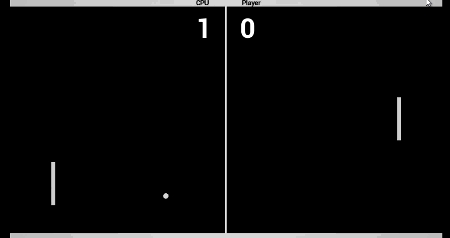
\includegraphics[width=\textwidth]{PongPhys}
\end{figure}

This screenshot from the environment shows main elements of the game:
\begin{enumerate}
    \item Paddles ---
        Every player controls a solid rectangle called paddle that can reflect the ball.
    \item Ball ---
        The ball is a rigid body that moves with a constant speed and reflects from the walls and paddles.
    \item Walls ---
        The walls are present on the top and on the bottom of the screen.
    \item Goals ---
        The left and right sides of the screen represent goals. In order to score a point, the player needs to hit the opposite goal with the ball.
    \item Scores ---
        The top part of the screen shows two numbers that are equal to the number of points each player have scored.
\end{enumerate}

The purpose of the game is to maximize the difference between your score and opponent score.

The human player uses raw pixels (screenshots) as an input during play, and outputs three types of actions using the keyboard:
\begin{itemize}
    \item Key up --- move paddle up
    \item Key down --- move paddle down
    \item Idle --- paddle stays at the same place
\end{itemize}

The game comes with the built-in AI controller that gets high-level features such as position and speed of the ball, position of his and opponent paddle as an input,
and uses rule-based approach to control the paddle.

\subsection{Python Scripting}

In Unreal Engine 4, the standard way to implement game logic is through writing C++ modules or using internal visual scripting language called Blueprints.
The C++ approach is more powerful and is used to implement core game logic and reusable modules, though in many cases it's overly verbose, and doesn't allow to quickly iterate on the solution due to slow compilation speeds.
On the other hand, blueprints are simple to create and understand, allow faster development cycles, yet not expressible enough in many cases.

When it comes to the modern machine learning engines, they are usually written in C++, while the public API that they provide comes in form of Python bindings.
While in principle it's possible to use TensorFlow C++ API, this approach limits the reuse of openly available RL algorithms implementations in Python, and slows down the research process due to the nature of the C++ language.

Due to all this reasons we looked into alternative languages support for UE4 and identified two candidates: Python and Lua.
Both languages are supported through third-party plugins available on GitHub, \href{https://github.com/facebook/UETorch}{UETorch} for Lua and \href{https://github.com/20tab/UnrealEnginePython}{UnrealEnginePython} for Python.

As the authors were more familiar with Python and TensorFlow, it was chosen as the primary language.
During this work, the original plugin was extended to support Python-based controllers in UE4.

The plugin allows users to write Python scripts that interact with UE4 engine by being able to access and mutate the internal state of the game.
This can be used to obtain current position of the ball and paddle, and giving the commands to move the paddle.

\subsection{RL Model}

We implement bot controller using TensorFlow machine learning framework \cite{tensorflow2015-whitepaper} to utilize GPU and multi-core CPU resources.
We use Deep Q-Network (DQN) \cite{mnih-dqn-2015} learning algorithm to train and control the bot.
The reward of +1 is given to the bot when it scores a point, and -1 when the opponent scores a point.

The bot is trained with fixed FPS 32. The screenshots are binarized and rescaled to resolution 80x80.

\subsection{Results}

We've built a Deep RL based controller that outperforms the standard rule-based bot, while using raw pixels as an input.
The training usually takes 6 hours on GPU and it takes 10 million iterations to beat the built-in scripted bot.

The code implementation is available on \href{https://github.com/akashin/HSE_AI_Labs/tree/master/Lab_4}{GitHub}.
